\chapter{Implementierung}
\label{chap:implementation}

Um die in Kapitel \ref{chap:threads} Probleme zu mindern oder gar zu beheben, kann eine Auswahl an vorgestellten Technologien (siehe \ref{chap:technologies}) genutzt werden. Die grundlegende Idee ist dabei der Schutz einer kleinen Anzahl von Clients durch den Einsatz eines speziell konfigurierten lokalen, rekursiven Resolvers. Es ist dabei nicht sinnvoll alle anwendbaren Techniken einzusetzen, da jede entsprechenden Kosten in Performance einhergeht und die Vorteile mancher Kombinationen redundant sind.

\section{Position und Resolver Typ}
Die möglichen Positionen und Betriebsarten eines Resolvers (siehe Abb. \ref{img:impl-resolverpositions}) wurden bereits im Abschnitt \ref{sec:dnsresolverposition} behandelt. Für die Auswahl wurden 3 Kriterien betrachtet: Angreifbarkeit, Performance und Privacy.
\begin{figure}[hb]
    \centering
    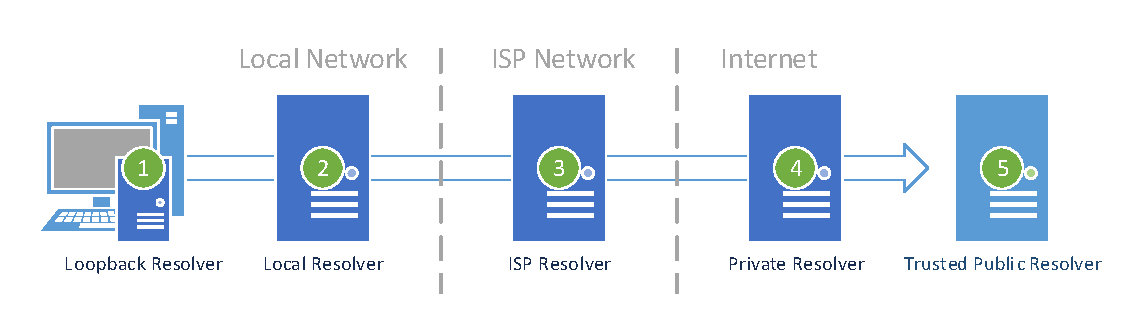
\includegraphics[width=\textwidth]{Impl_ResolverPositions}
    \caption{Stellt die möglichen Positionen eines Resolvers, aus Sicht des Clients, dar.}
    \label{img:impl-resolverpositions}
\end{figure}

\paragraph{Local-Loopback Resolver (1)}
Diese Position ist bei einem, auf die Verbindung zwischen Recursive Resolver und Stub-Resolver abgezielten, Angriff die sicherste, da diese Kommunikation nicht über das Netzwerk passiert. Je nach Betriebsmodus, Forwarding oder Recursive, kann die Kommunikation zu den nachgereihten Servern sehr wohl attackiert werden. In wie fern das ein Problem ist, hängt von dem verwendeten Protokoll ab. Der klare Vorteil besteht beim Einsatz von Techniken wie DoT,DoH oder DNSCrypt in Forwarding Modus da somit die Vertraulichkeit und Authentizität bis zum Recursive Resolver gegeben sind. Nachteil ist die fehlende Möglichkeit eines über Hosts geteilten Cache, die notwendige Performance und der hohe Wartungsaufwand. Außerdem können keine IoT-Geräte bedient werden, da bei diesen eine Installation eines lokal laufenden Resolvers nicht möglich ist.

\paragraph{Local Network Resolver (2)}
Durch einen Resolver im Lokalen Netzwerk, wird zwar die Möglichkeit von Angriffen auf Netzwerkebene gegeben, dafür gewinnt man jedoch die Möglichkeit des gemeinsamen Caches und eine hohe Geräte-Kompatibilität. In kleinen, gut gewarteten Netzwerken, mit einer Firewall am Netzwerkübergang, kann aufgrund des geringen Risikos von Angriffen auf die Stub-Resolver zu Resolver Verbindung abgesehen werden. Angriffe von außen sind jedoch durchaus möglich und wahrscheinlich.

\paragraph{ISP Resolver (3)}
Da, wie in Abschnitt \ref{sec:thread-priv} beschrieben, nicht auf die Verantwortlichkeit von ISPs oder staatlichen Institutionen vertraut werden sollte, ist das Nutzen eines ISP-Resolvers, vor allem in Hinblick auf Privacy, nicht zu empfehlen. Einzige Ausnahme stellt dabei der Einsatz von Technologien wir DNSCurve, EncDNS und ODNS dar. Da diese eine Verschlüsselung der Anfragen durch den Resolver hindurch unterstützen. Aufgrund kurzer Laufwege und großen Caches sind diese Resolver in den meisten Fällen durchaus performant.

\paragraph{Private Resolver (4)}
Betreibt man seinen eigenen Resolver im Internet ist der Hauptvorteil, dass man dadurch Kontrolle über die Privacy-Einstellungen des Resolvers hat. Abgesehen davon, setzt man sich damit auch allen Gefahren aus, die das Angriffsspektrum, nicht nur auf DNS, zu bieten hat. Darüber hinaus sind die meisten Stub-Resolver nicht dazu in der Lage über sichere Protokolle mit dem Resolver zu kommunizieren. Hinzu kommt noch das Problem, dass es überaus Schwierig ist die richtige Zugriffsbeschränkung zu wählen. Bei einer zu weit gegriffenen Einschränkung, ist es einfach den Resolver als DoS-Amplifier zu missbrauchen. Bei einer zu engen Beschränkung ist eine direkte Zuordnung zwischen Server und Client möglich. Da abgesehen von Privacy, keine Vorteile gegenüber Public Resolvern bestehen, kann vom Einsatz eines eigener, privater Resolvers abgeraten werden.

\paragraph{Public Resolver (5)}
Der direkte Einsatz eines Trusted Public Resolvers hat viele Vorteile. Die Performance ist aufgrund guter Anbindungen, eines professionellen Betriebs und großen Caches meist überdurchschnittlich gut. Viele Resolver haben spezielle Schutzmaßnahmen gegen Cache Poisoning- oder DoS-Attacken im Einsatz. Außerdem ist die Anonymisierung aufgrund der hohen Zahl an Users als ausreichend anzusehen. Der einzige, schwerwiegende Nachteil besteht in der Gefahr von Privacy-Verletzungen durch den Betreiber des Dienstes. Hier ist entweder eine Abwägung zu treffen oder eine Lösung zur Anonymisierung zu finden. 

\section{Technologie-Stack}
Zur Auswahl des Sets an Technologien, hier als ``Stack'' bezeichnet, wurde aufgrund der am Ende des Kapitels \ref{chap:attacks} angeführten Übersicht erstellt. Dabei wurde darauf geachtet, jede der unter \ref{chap:solutions} abgegebenen Empfehlungen gerecht zu werden. Um die Auswahl besser verstehen zu können, wird hier kurz auf jede einzelne der Techniken eingegangen.

\paragraph{DNSSEC}
DNSSEC stellt aktuell die einzige Möglichkeit zur Echtheitsprüfung der Records selbst dar (siehe Abschnitt \ref{sec:tec-dnssec}). Das Abfragen und Validieren der DNSSEC Signatur-Records ist somit Pflicht für jeden Resolver mit Sicherheitsfokus. Die Validierung kann an verschiedenen Stellen erfolgen. Da die Validierung aufgrund der kryptographischen Operationen durchaus Performanceintensiv sein kann, ist es Sinnvoll diese Operation nicht auf jedem Client durchzuführen. Abgesehen davon fehlt vielen Stub-Resolvern die Möglichkeit zur selbstständigen Validierung. Wird ein Forwarding-Resolver eingesetzt, kommt es auf die Konfiguration und Implementierung an ob dieser eine Validierung durchführt oder sich auf den nachgeordneten Recursive Resolver verlässt. Kann dem rekursiven Resolver vertraut werden, ist die Verifizierung durch diesen, aus effizienzgründen, zu bevorzugen.

\paragraph{DNS-over-TLS}
Wie in Abschnitt \ref{sec:tec-dot} beschrieben stellt DoT einen simplen Aufsatz um klassischen DNS Netzwerkprotokoll dar. Für den Transport wird TLS über TCP auf Port 853 genutzt \cite{rfc7858}. Damit ist die Vertraulichkeit der Verbindung zwischen Resolver und Recursive Resolver geschützt. 

\paragraph{Address-Obfuscation über NAT}
Um auch die Vertraulichkeit der Anfragen erhalten zu können, ist es wichtig den Zusammenhang zwischen der Client-Adresse und der Anfrage aufzulösen. Dies kann, wie schon in Abschnitt \ref{sec:tec-nat} erwähnt, durch den Einsatz eines NAT Servers erreicht werden. Dies kann mit nahezu jedem modernen Server-Betriebssystem realisiert werden.

\section{Konzept}
Aus den beschriebenen Vor- und Nachteiler der Position eines Resolvers bzw. dessen Betriebsmodus ergibt sich, dass es vernünftig ist, einen Lokalen Forward Resolver einzusetzen. Der beschriebene Technologie-Stack ist darüber hinaus in der Lage alle in Kapitel \ref{chap:solutions} vorgestellten Empfehlungen zu folgen. In Abbildung \ref{img:impl-architecture} wird der schematische Ablauf der Kommunikation gezeigt. Es werden dabei zusätzlich die Übergangsstellen der Verschlüsselung und Client-Identifizierbarkeit gezeigt.

\begin{figure}[hb]
    \centering
    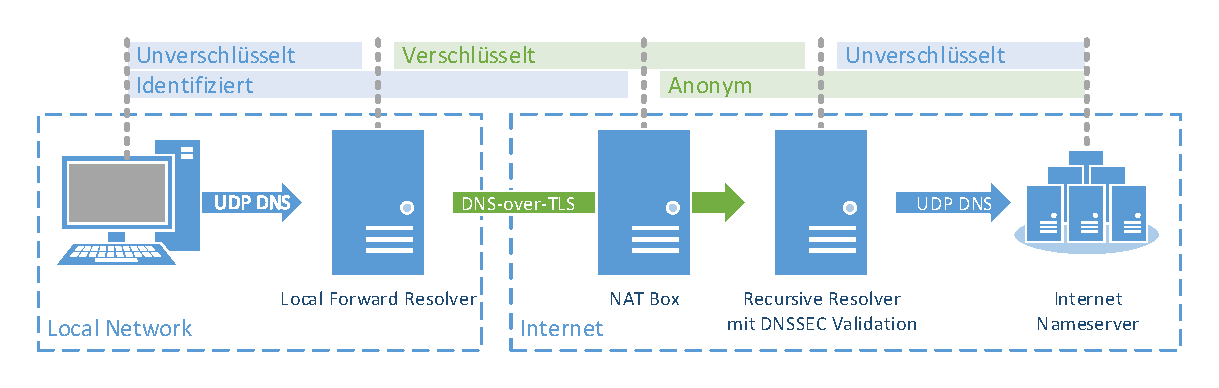
\includegraphics[width=\textwidth]{Impl_Architecture}
    \caption{Darstellung des schematischen Kommunikationsweg des Test-Aufbaus.}
    \label{img:impl-architecture}
\end{figure}

Um die Privacy der lokalen Clients und damit der Nutzenden zu wahren, wurde der Aufbau nach einer, durch EncDNS \cite{Herrmann2014} inspirierten, Grundkonzept entworfen: Entschlüsselte DNS-Anfragen oder Antworten dürfen nur, auf vom User direkt kontrollierten Komponenten, mit der externen Internet-Adresse verknüpfbar sein. Dadurch wird verhindert, dass Betreiber der Transportnetzwerke oder der nachgeordneten DNS-Komponenten private Daten mit der Identität der Nutzenden verknüpfen.

Des weiteren wird durch die eingesetzte Verschlüsselung jede Form von Sniffing und Spoofing Attacken (siehe Kapitel \ref{chap:attacks}) unmöglich gemacht. Da der Forwarding-Resolver selbst keine Anfragen von außerhalb des lokalen Netzwerks annimmt, ist der Resolver auch gegen DNS DoS Attacken durch externe Angreifer geschützt. Die DNSSEC Validierung erfolgt je nach Implementation am lokalen Forward Resolver oder am Public Recursive Resolver, in jedem Fall werden dem Client jedoch Informationen zum Validierungsstatus der Antworten geliefert. Es ist damit selbst im Falle einer erfolgreichen Cache-Poisoning Attacke des Public Resolvers nicht möglich RRs zu kompromittieren die durch DNSSEC Signaturen geschützt sind.

\section{Aufbau}
\label{sec:architecture}
Zu Validierung des Entwurfs wurde ein einfacher Testaufbau realisiert. Dieser verwendet Windows 10\footnote{Microsoft Windows Version 1803 (Build 17134.285)} als Test-Client-Betriebssystem und Fedora 28\footnote{Linux 4.17.19-200.fc28.x86\_64} als Betriebssystem des lokalen Resolvers. Der Local-Resolver selbst wurden zwecks Vergleichbarkeit mit zwei verschiedenen Software-Paketen umgesetzt: Unbound 1.7.3\footnote{Kompiliert mit OpenSSL 1.1.0h-fips} und Knot-Resolver 2.4.1. Als Trusted Public Resolver wurde das Quad9-Projekt gewählt, da es DoT anbietet und einer zu befürwortende Privacy-Policy\cite{Quad9Privacy} folgt. Darüber hinaus werden Domänen, die in Zusammenhang mit Schadsoftware stehen, automatisch geblockt. Dieses Feature kann zwar als Zensur verstanden werden, durch die aktuelle Bedrohung durch DNS unterstützte Malware \cite{Alcoy2017} und die strikt auf ``Phishing, Malware, and Exploit-Kits'' konzentrierte Sperrliste\cite{Quad9FAQ} überwiegen die Vorteile jedoch diesem Risiko.   

\begin{figure}[!hb]
    \centering
    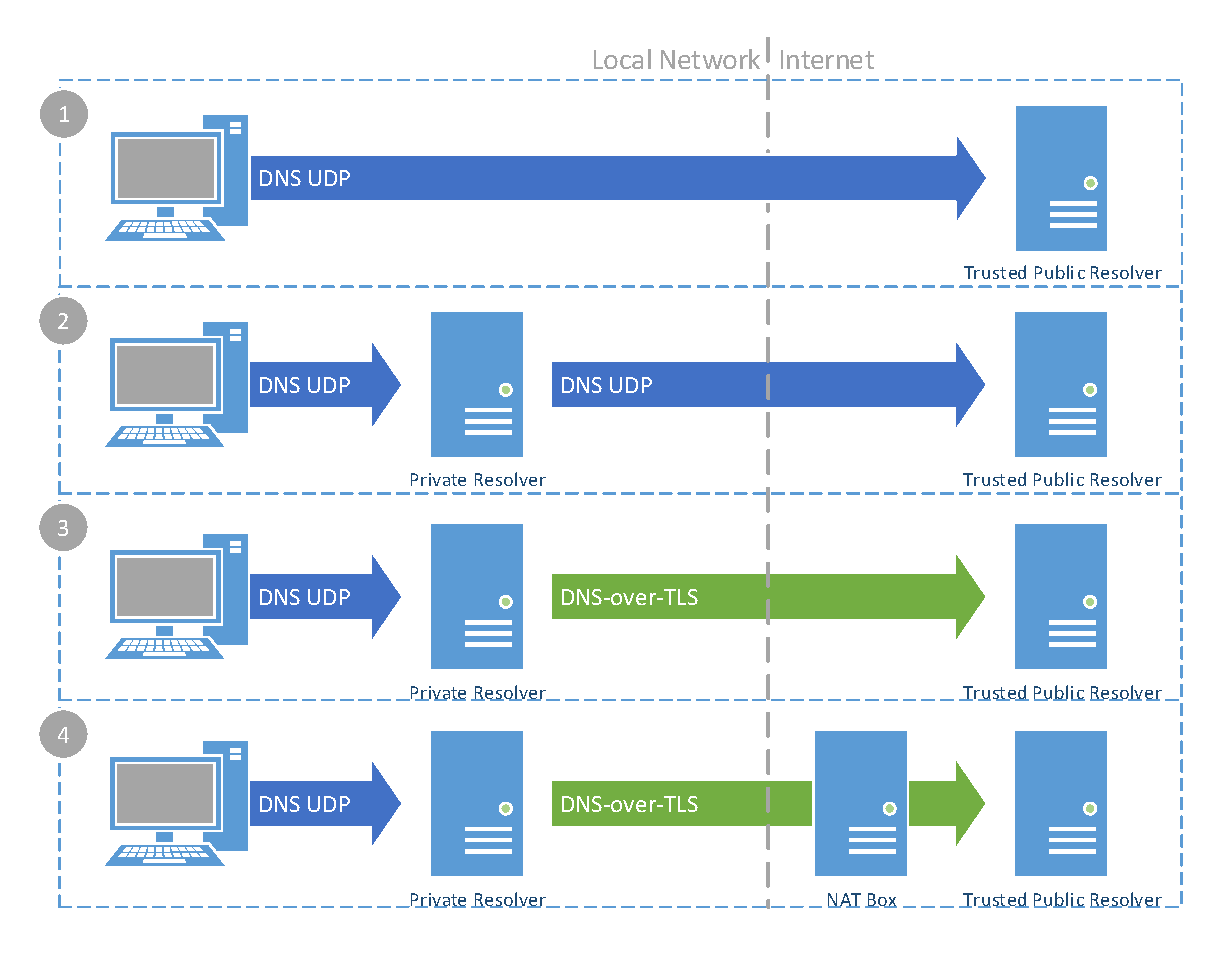
\includegraphics[width=\textwidth]{Impl_Scenarios}
    \caption{Darstellung der getesteten Szenarien}
    \label{img:impl-scenarios}
\end{figure}

Wie in Abbildung \ref{img:impl-scenarios} dargestellt wurden für den Performance- und Funktions-Test 4 Szenarien gewählt. Dabei erfüllt nur Szenario 4 alle beschriebenen Schutzmechanismen, wobei Szenario 3 nur die Anonymität gegenüber des Public Resolver verletzt. Geht man von einem vertrauenswürdigen Anbieter dieses Resolvers aus, kann auf die Anonymisierung über den NAT-Server verzichtet werden. Wie man sieht, wird in jedem Fall von einem sicheren lokalen Netzwerk ausgegangen, mögliche Lösungen bei unsicheren Netzwerken wir in Kapitel \ref{chap:future} diskutiert. 

\paragraph{Public-Resolver über UDP (1)}
Durch die direkte Verbindung zwischen Stub-Resolver und Public Resolver wird auf jegliche Vertraulichkeit der Übertragung verzichtet, da der in Windows integrierte Stub-Resolver keine Form der Verschlüsselung unterstützt. Abgesehen davon, ergibt sich durch die minimale Anzahl an Zwischenstellen eine optimale Latenzzeit, die sich positiv auf die gesamte Performance auswirkt.

\paragraph{Lokalen Forwarding-Resolver über UDP (2)}
In diesem Fall wird ein Forwarding-Resolver im lokalen Netzwerk installiert. Da dieser aber das klassische DNS-Netzwerkprotokoll zur Kommunikation mit dem Recursive Resolver verwendet, ergibt sich noch kein Schutz der Vertraulichkeit. Mit einer restriktiven Konfiguration und verschiedenen, von der Implementation abhängigen, Sicherheitsfeatures können jedoch gewisse Arten von Spoofing-Attacken ausgeschlossen werden. Befindet sich eine Firewall an der Netzwerkkante so kann diese durch den Einsatz eines lokalen Resolvers sehr restriktiv Eingestellt werden. Dies verhindert direkte Angriffe auf Stub-Resolver von extern. Ein weiterer Vorteil besteht beim Einsatz von ``Knot-Resolver'' da dieser bestimmte DNS Rebinding Attacken (siehe \ref{sec:attack-dnsrebind}) abwehren kann, indem er interne IP-Adressen in Antworten verbietet\cite{KnotResolverDocRebinding}.

\paragraph{Lokaler Forwarding-Resolver mit DoT (3)}
Wird die Verbindung zum Recursive-Resolver nun durch ein Verschlüsselungsprotokoll wie DoT (siehe \ref{sec:tec-dot}) geschützt, ergeben sich ein klarer Vorteil: Es besteht volle Vertraulichkeit zwischen dem Forwarding- und Recursive-Resolver, was Sniffing-, Spoofing-, sowie MITM-Attacken auf diesem Wege ausschließt. Durch den Einsatz von verbindungsorientierten Protokollen und Verschlüsselung werden auch Nachteile in Performance und Latenzzeit merkbar.

\paragraph{Lokaler Forwarding-Resolver mit DoT und NAT (4)}
Fügt man dem Aufbau nun einen NAT-Server (siehe \ref{sec:tec-nat}) hinzu, erhält man den Vorteil der Anonymität gegenüber des Recursive-Resolvers. Da dies der einzige Vorteil des Aufbaus darstellt, ist die dadurch einhergehende Erhöhung der Latenzzeit gegen das Schutzbedürfnis der Nutzenden abzuwägen.

\section{Tests und Messungen}
\label{sec:measurements}
Die Kontrolle der unter \ref{sec:architecture} beschriebenen Varianten wurde nun mithilfe der Programme DIG\footnote{Auf Ubuntu Subsystem for Windows10; DiG 9.10.3-P4-Ubuntu} sowie ``DNS Benchmark''\footnote{von Steve Gibson Version 1.3.6668.0} durchgeführt. Die gewählten Konfigurationen sind in \nameref{chap:appA} zu finden und wurden nach den offiziellen Dokumentationen und darin enthaltenen Sicherheitsempfehlungen erstellt. Als ``Hardware'' wurden 3 virtuelle Maschinen (1 vCPU, 1GB RAM) auf einem vom Test-Client unabhängigen Host genutzt. Um eine optimale Vergleichbarkeit der einzelnen Varianten zu erreichen wurden die Test der Performance von einem Test-Client auf die 3 Server simultan durchgeführt. Dabei wurden in 2 unabhängigen Läufen alle unterschiedlichen Varianten einer Software getestet. In einem dritten Lauf wurde die direkte Performance von 25 offener DNS-Resolvern (siehe \ref{chap:appB}) getestet und die 10 besten zur Errechnung der direkten Vergleichswerte herangezogen. Für die Auswertungen wurden immer nur Werte von ungecachten Einträgen herangezogen, da nur diese eine Kommunikation mit dem Recursive-Resolver verlangen. Die Ergebnisse der Tests sind unter Kapitel \ref{chap:results} angeführt. 

